\documentclass[letterpaper, 11pt]{article} 

\usepackage{graphics,graphicx}
\usepackage{multicol} 
\usepackage{parskip}
\usepackage{amsmath}
\usepackage{multirow}
\usepackage[utf8]{inputenc}
\usepackage{fancyhdr}
\usepackage[title]{appendix}
\usepackage{wasysym}
\usepackage{url}
\usepackage{subcaption}

\usepackage[font=footnotesize,labelfont=small]{caption}
\captionsetup{width=0.85\linewidth}

\RequirePackage{geometry}
\geometry{margin=2cm}

\setlength{\parskip}{0.2cm}
\setlength{\parindent}{0pt}


\title{Assignment 2: Neural Coding}
\author{
Tai Duc Nguyen \\
BMES T580: Systems Neuroscience in Medicine and Engineering
}
\date{\today}

\begin{document}

\maketitle

\rule{\textwidth}{1pt}

\section{Problem 1}
\label{sec:prob1}
\textbf{Problem statement:} Answer the following questions:

a. Please describe the response of each of the cell-type when the photoreceptor is stimulated by a brief pulse of light that is large enough to affect all the bipolar cells. Your response should include a sketch as if you are performing whole-cell patch clamp recording from these neurons, and a short description why you expect a particular response.

b. Same as A except that the light is turned off. Essentially, a steady light is turned off and then on to the same level.

c. What is the optimal stimulus for this ganglion cell? 

d. In class, we discussed two kinds of ganglion cells: “pixel detectors” and “feature detectors”. Which class of ganglion cell does this neuron belong to? Explain, please.

\textbf{Answer:}

\begin{figure}[htb!]
	\centering
	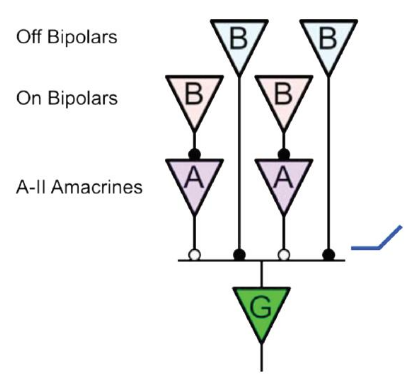
\includegraphics[width=0.5\linewidth]{fig1.png}
	\caption{}
	\label{fig1}
\end{figure}

a. If the photoreceptors connecting to these bipolar cells are stimulated by a brief pulse of light:
\begin{itemize}
	\item The Off Bipolars will send inhibitory response.
	\item The On Bipolars will send excitatory response.
	\item The AII Amacrines will receive excitations from the On Bipolar and inhibit its reponse.
	\item Since the signals connecting to the Ganglion cell are linearly rectified, the inhibition from the AII Amacrines and Off Bipolars will just be 0. Hence, the signal from the Ganglion will just be a flat line.
\end{itemize}

b. If the steady light in A is turned off:
\begin{itemize}
	\item The Off Bipolars will send excitatory response,
	\item The On Bipolars will send inhibitory response.
	\item The AII Amacrines will receive inhibitions from the On Bipolar and NOT inhibit its reponse.
	\item The Ganglion cell will emit a strong positive signal due to receiving 4 excitatory signals.
\end{itemize}

c. From part B, since all signals connecting to the Ganglion cells are excitatory, the stimulus in B should give the highest (hence, optimal) amount of stimulus.

d. This Ganglion cell is a pixel detector because it outputs a no response when there is light and no response when it's dark.


\section{Problem 2}
\label{sec:prob2}
\textbf{Problem statement:} The figure below shows two linear filters belonging to two different retinal neurons. Answer the following: 

a. What kind of neurons would have such a linear filter? Explain

b. If everything else remains the same, draw the responses of these neurons to a 100 ms(millisecond) pulse of light?

\begin{figure}[htb!]
	\centering
	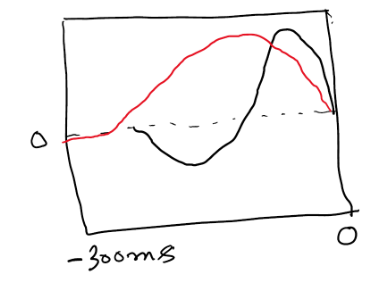
\includegraphics[width=0.5\linewidth]{fig2.png}
	\label{fig2}
\end{figure}

\textbf{Answer:}

a. The red line is describing a bipolar cell because:

The red linear filter describes a system where the stimuli at t $\approx$ 200 to 0 ms are weighted positive and higher than other stimuli at different t. The dot product of this filter and a stimulus signal will only result in a positive number. Hence, this can be similar to a bipolar cell passing on signals from photoceptors.

The black line is a ganglion cell because:

The black linear filter describes a system where the stimuli at t  $\approx$ 200 to 100 ms are weighted negatively and the stimuli at t  $\approx$ 100 to 0 ms are weighted positively. The dot product of this filter and a stimulus signal can result in a positive or a negative number. Therefore, this is analogous to a retinal ganglion cell receiving inhibitions from an amacrine cell and exitation from a bipolar cell.

b. The responses to a 100ms pulse of light is shown in the figure below

\begin{figure}[htb!]
	\centering
	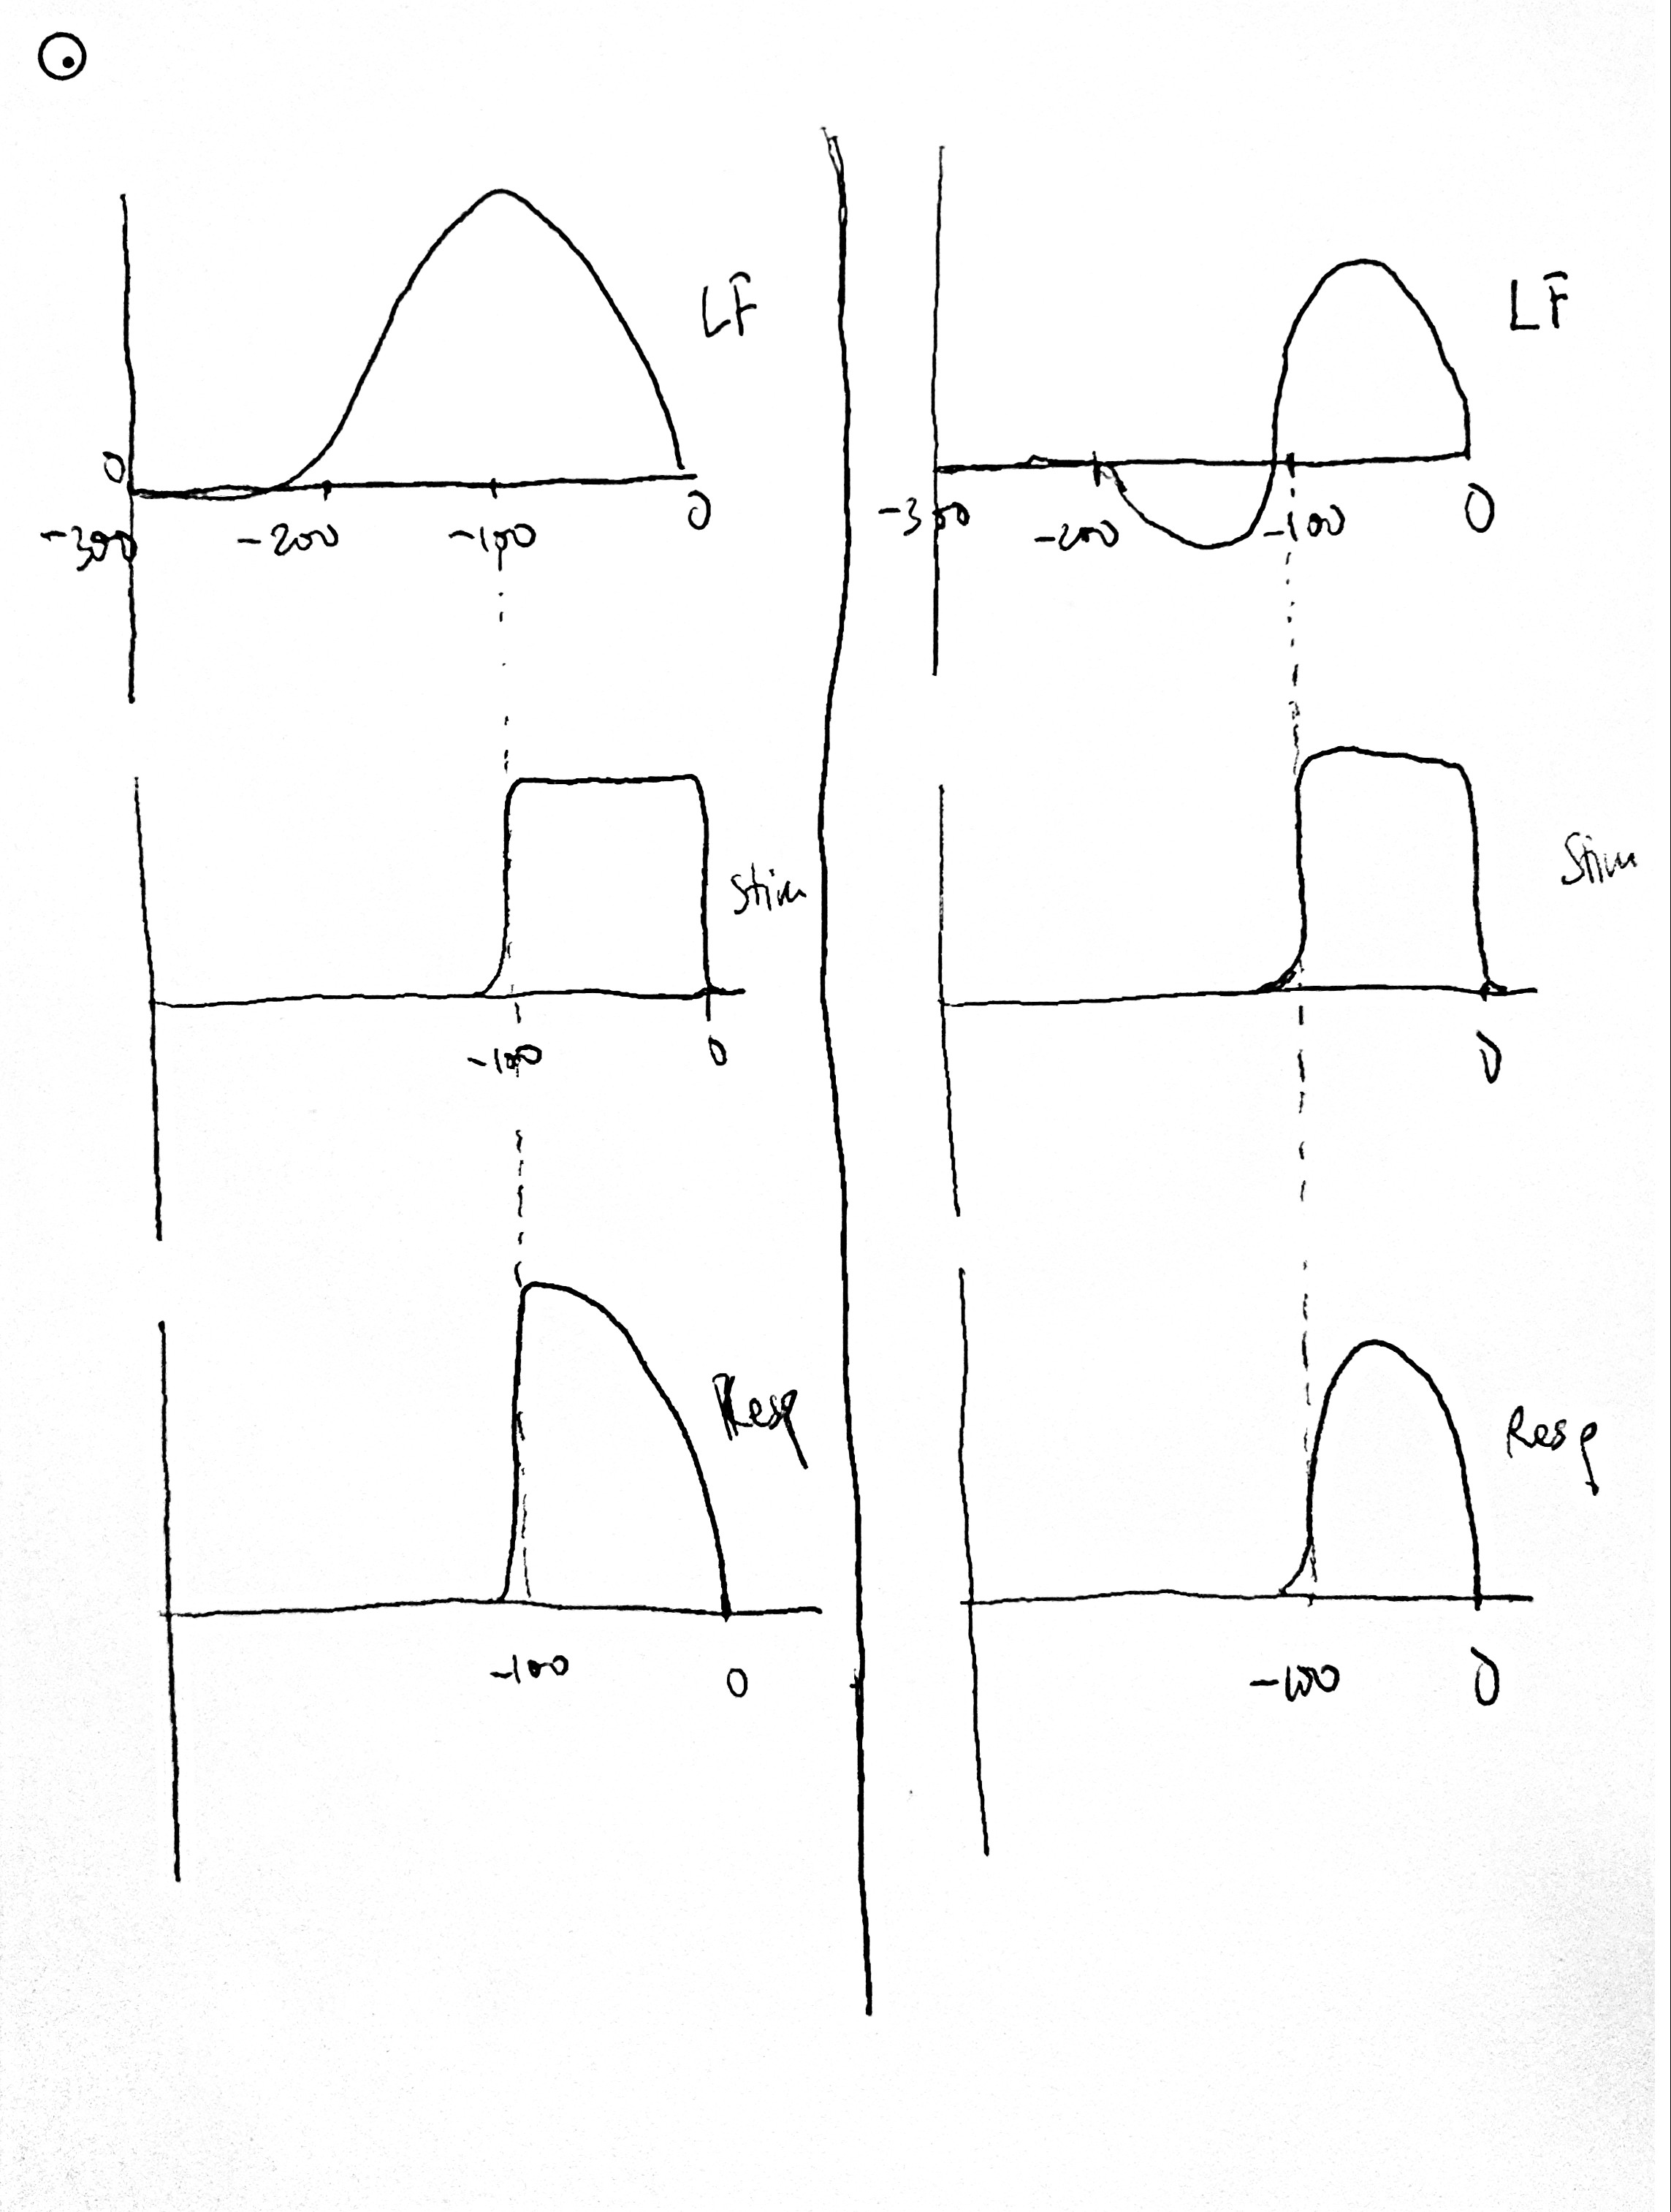
\includegraphics[width=0.5\linewidth]{2.jpg}
\end{figure}

\section{Problem 3}
\label{sec:prob3}
\textbf{Problem statement:} Responses to two neurons to two drifting grating stimuli are shown below. These neurons are from the same brain region. Answer the following questions:

a. What kind of recording is being performed here? Explain your response.

b. What is the key difference between these neurons. Explain your response.

c. What kind of cells (i.e. which brain region and cell-type) are being recording from here? Explain your response.

\begin{figure}[htb!]
	\centering
	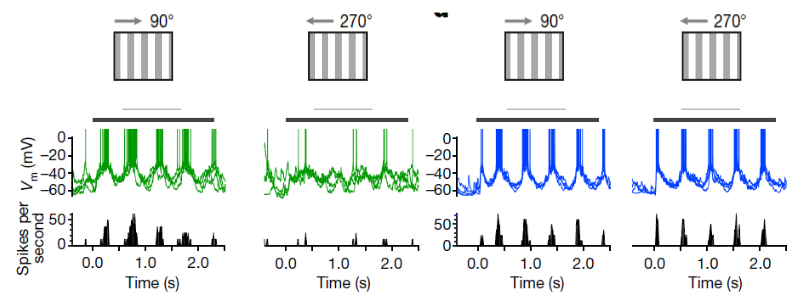
\includegraphics[width=0.8\linewidth]{fig3.png}
	%	\caption{DFF's Layout in Cadence's Virtuoso Layout Suite}
	\label{fig3}
\end{figure}

\textbf{Answer:}

a. The recording being performed here is extracellular because the researchers producing this figure are mostly interested in the number of spikes, rather than measuring macroscopic currents in a neuron. Also, the recording looks very noisy, which means it would only be good when counting spikes over a period of time.

b. The green neuron is directionally sensitive with a preferred direction because: 
\begin{itemize}
	\item When the grating is moving from left to right, \textbf{it reponses with spikes of approximately the same phase as the stimulus. }
	\item When the grating is moving from right to left, \textbf{the response is much WEAKER and NOT in the same phase as the stimulus.}
\end{itemize}

The blue neuron is not directionally sensitive because: 
\begin{itemize}
	\item Despite the change in the direction of the grating movement, the neuron seems to spikes at the same rate with the same phase.
\end{itemize}

c. These two cells are in the primary visual cortex (V1) region of the brain. The green one is likely a complex cell and the blue one is likely a simple cell. This observation is due to the fact that the green neuron is able to differentiate the direction of movement, while the blue neuron can't.


\section{Problem 4}
\label{sec:prob4}
\textbf{Problem statement:} This is a correlation or Reichardt motion detector. In class notes, you will find a detailed account of how each stage of the one-half of the motion detector will respond to a moving bar. Based on the notes, answer the following:

a. Draw the response at each stage of the “complete” motion detector to a moving bar

b. How would the response change if you replace the moving bar with a moving grating

\begin{figure}[htb!]
	\centering
	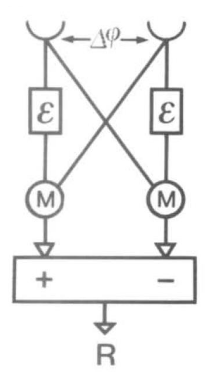
\includegraphics[width=0.2\linewidth]{fig4.png}
	%	\caption{DFF's Layout in Cadence's Virtuoso Layout Suite}
	\label{fig4}
\end{figure}

\textbf{Answer:}

a. The response to a moving bar of the motion detector is as follows

\begin{figure}[ht!]
	\centering
	\begin{subfigure}[b]{.45\linewidth}
		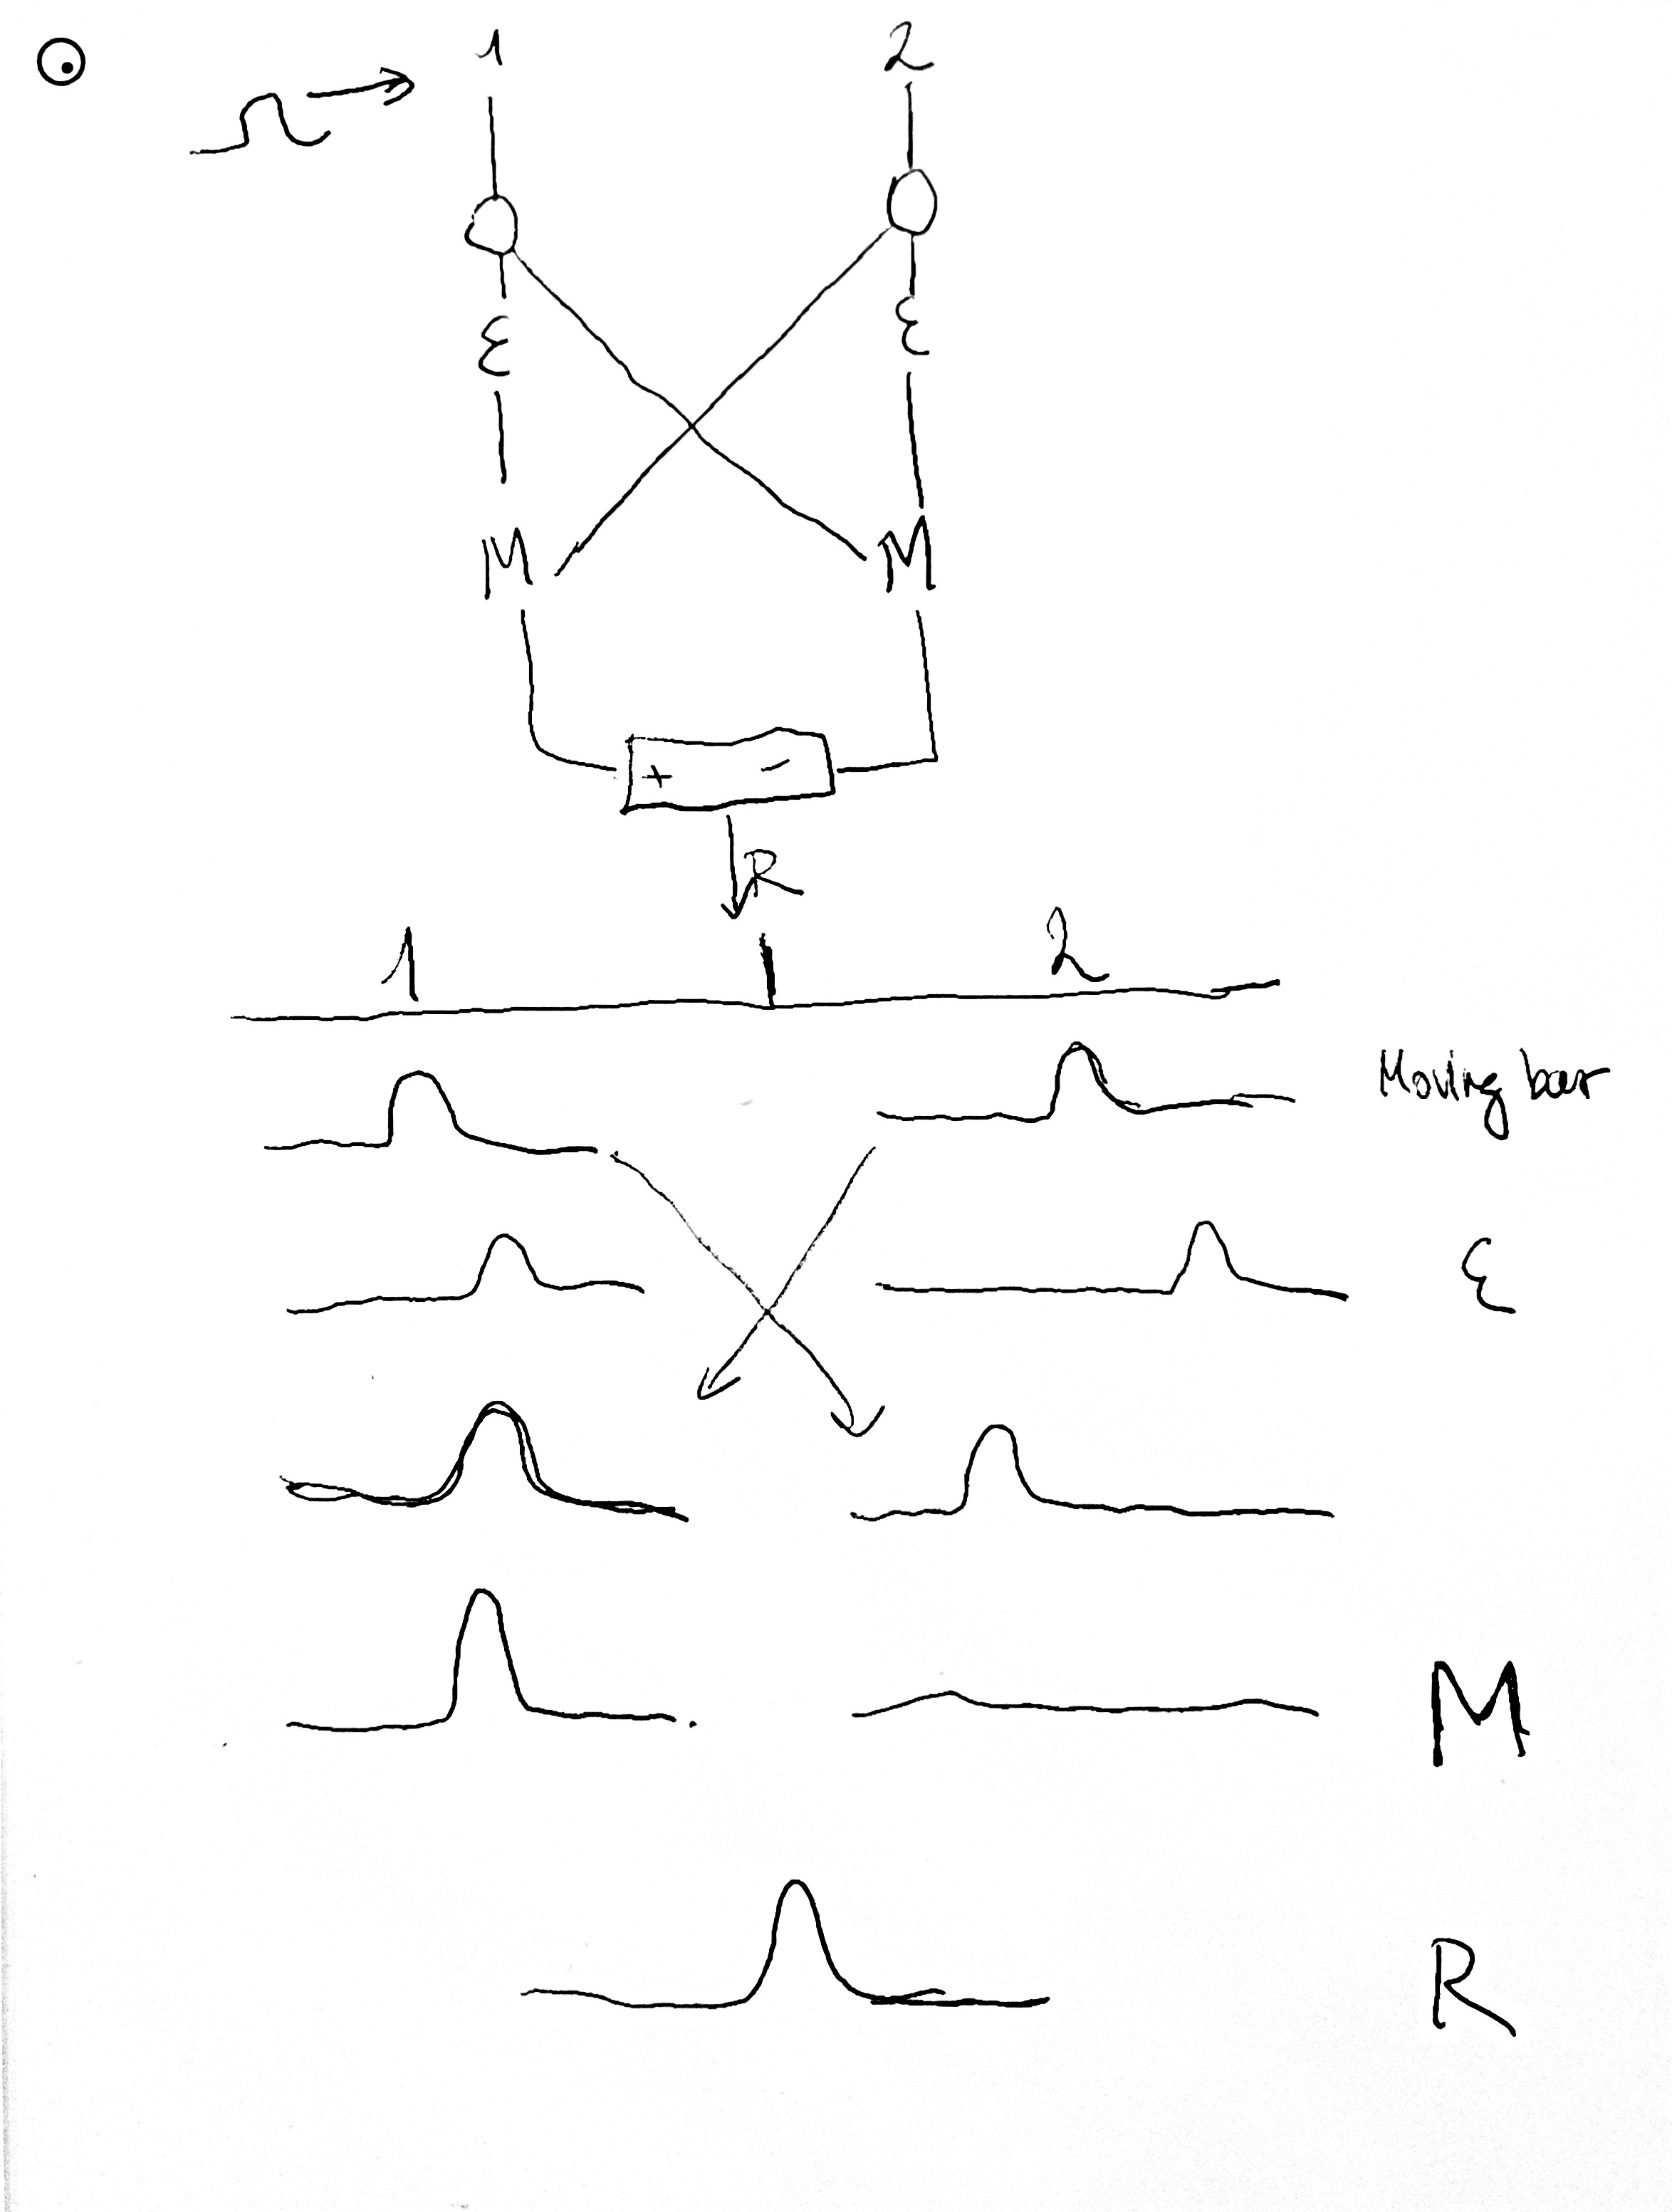
\includegraphics[width=\textwidth]{4a.jpg}
	\end{subfigure}
		\hskip2em
	\begin{subfigure}[b]{.45\linewidth}
		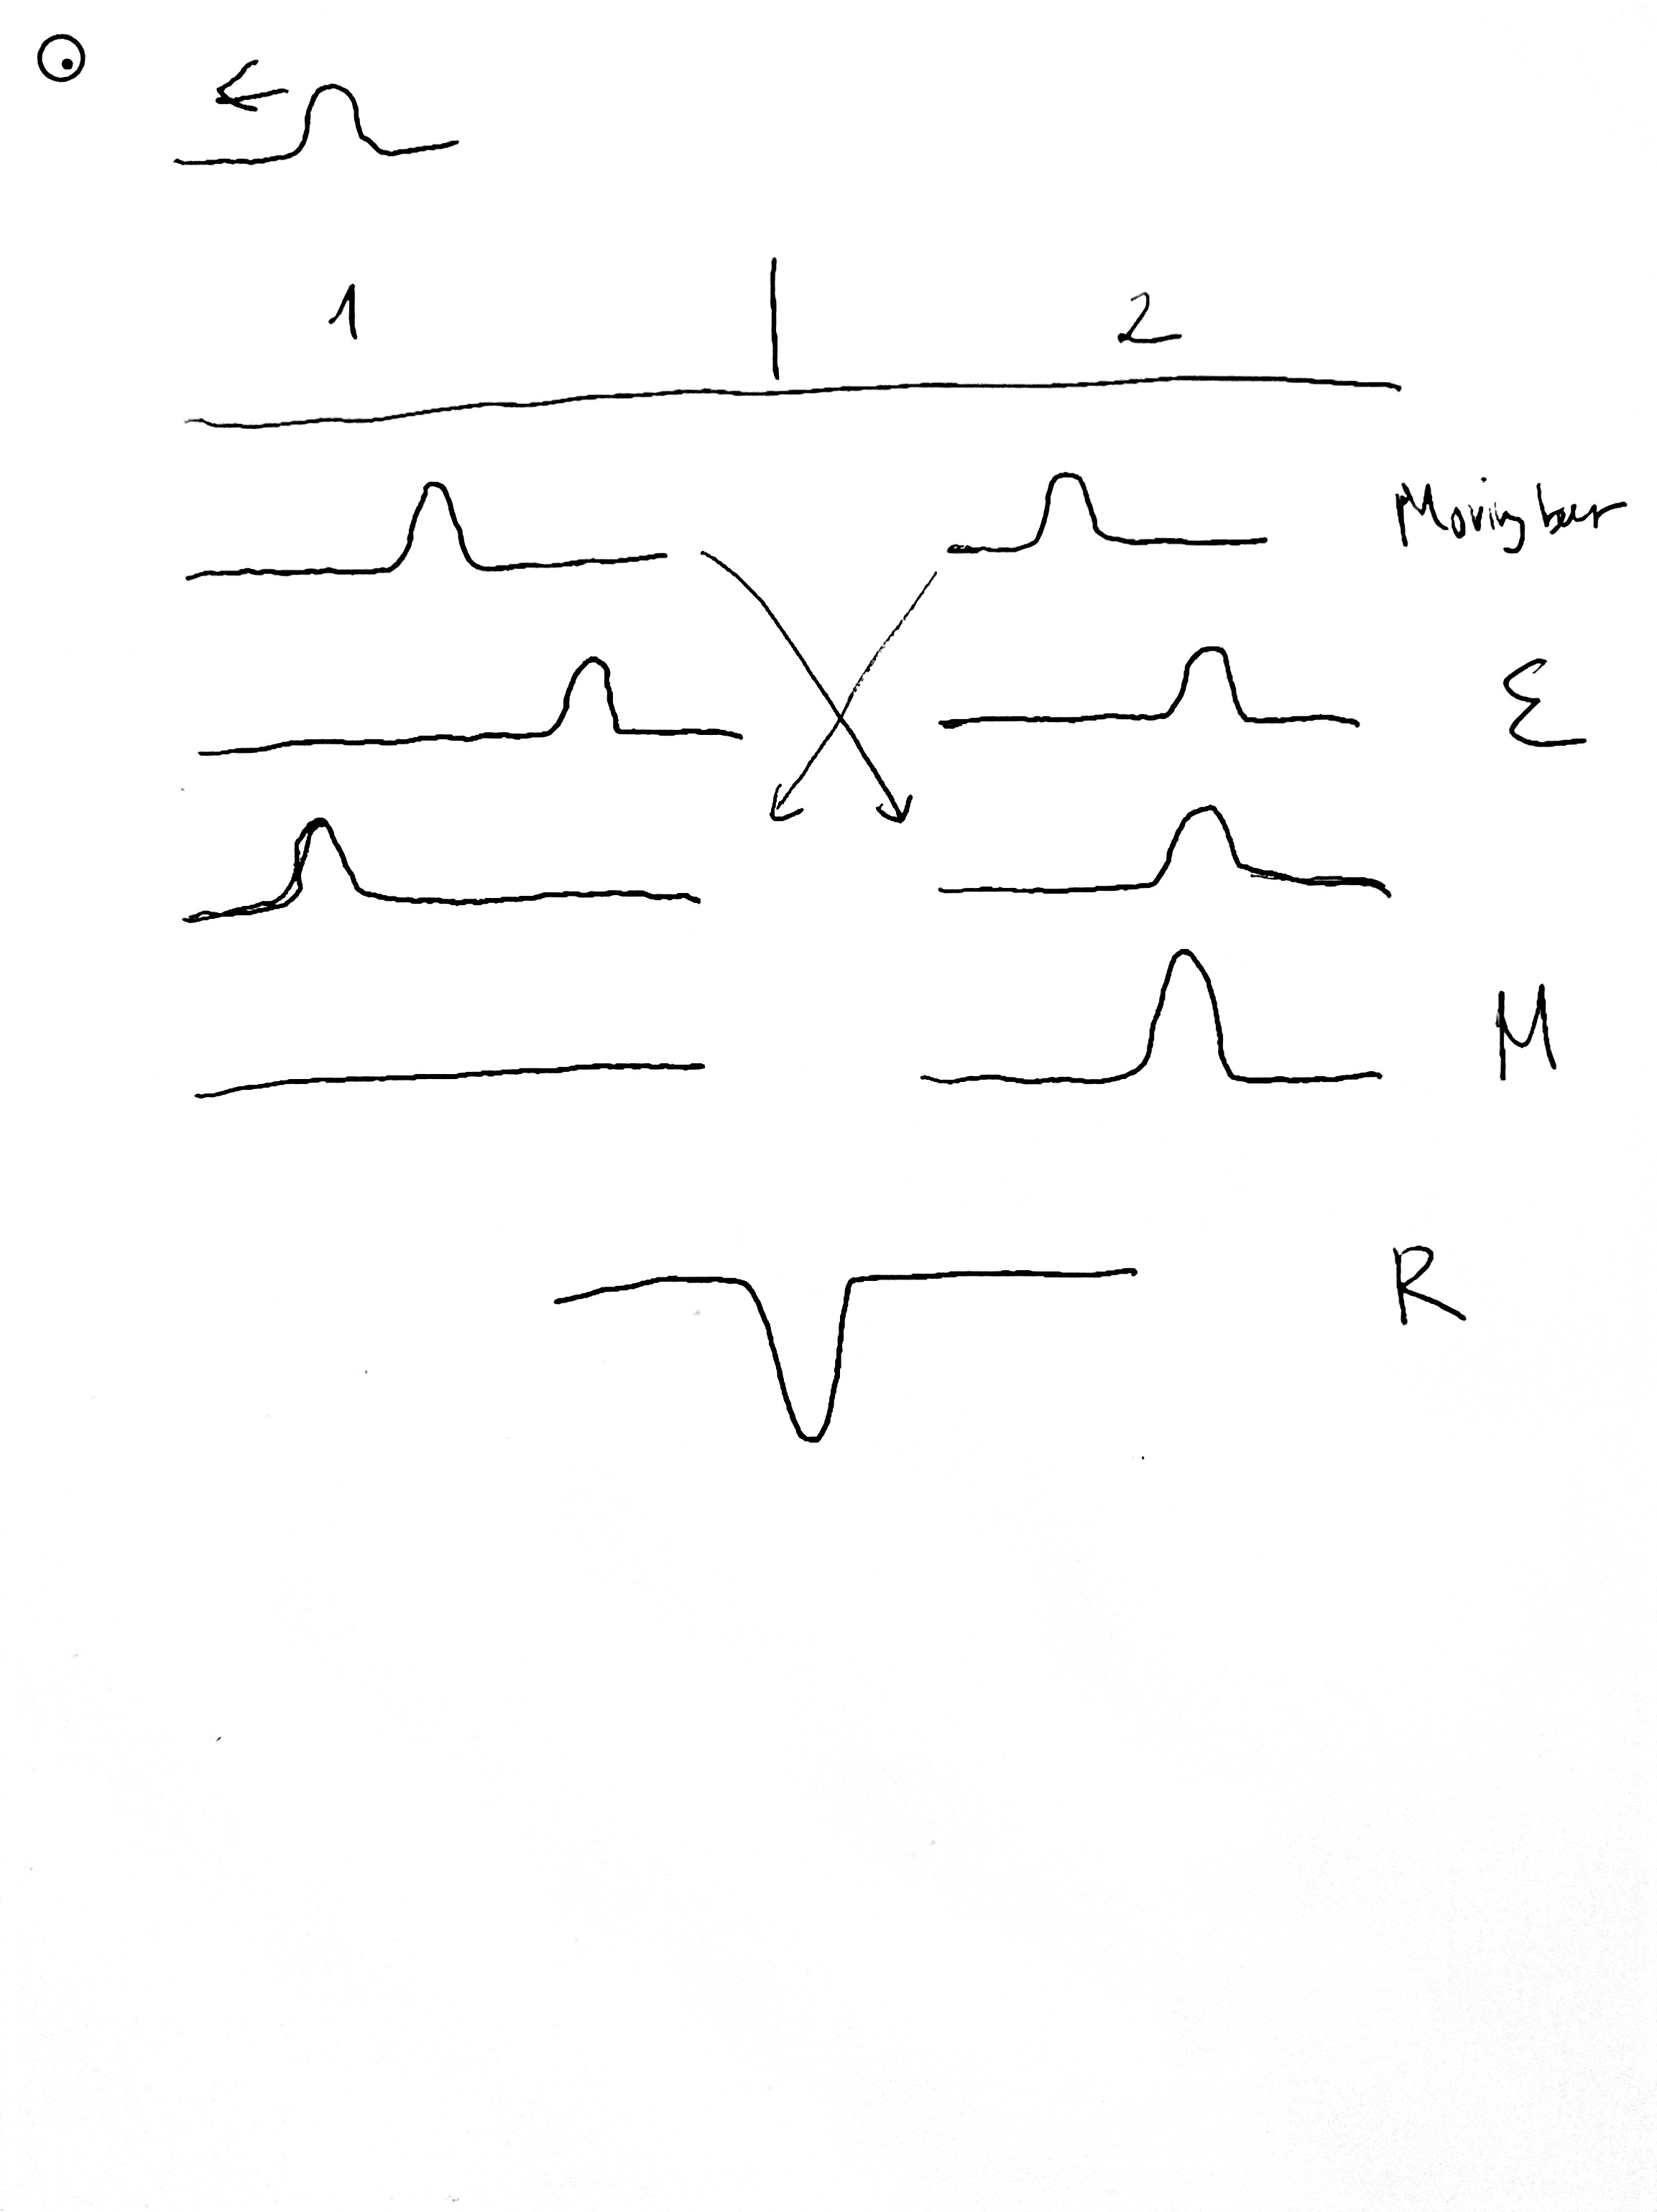
\includegraphics[width=\textwidth]{4b.jpg}
	\end{subfigure}
\end{figure}

\newpage

b. The repsonse to a moving grating will just be a oscillatory one with the same frequency as the stimulus but shifted due to delay in signal processing.

\begin{figure}[htb!]
	\centering
	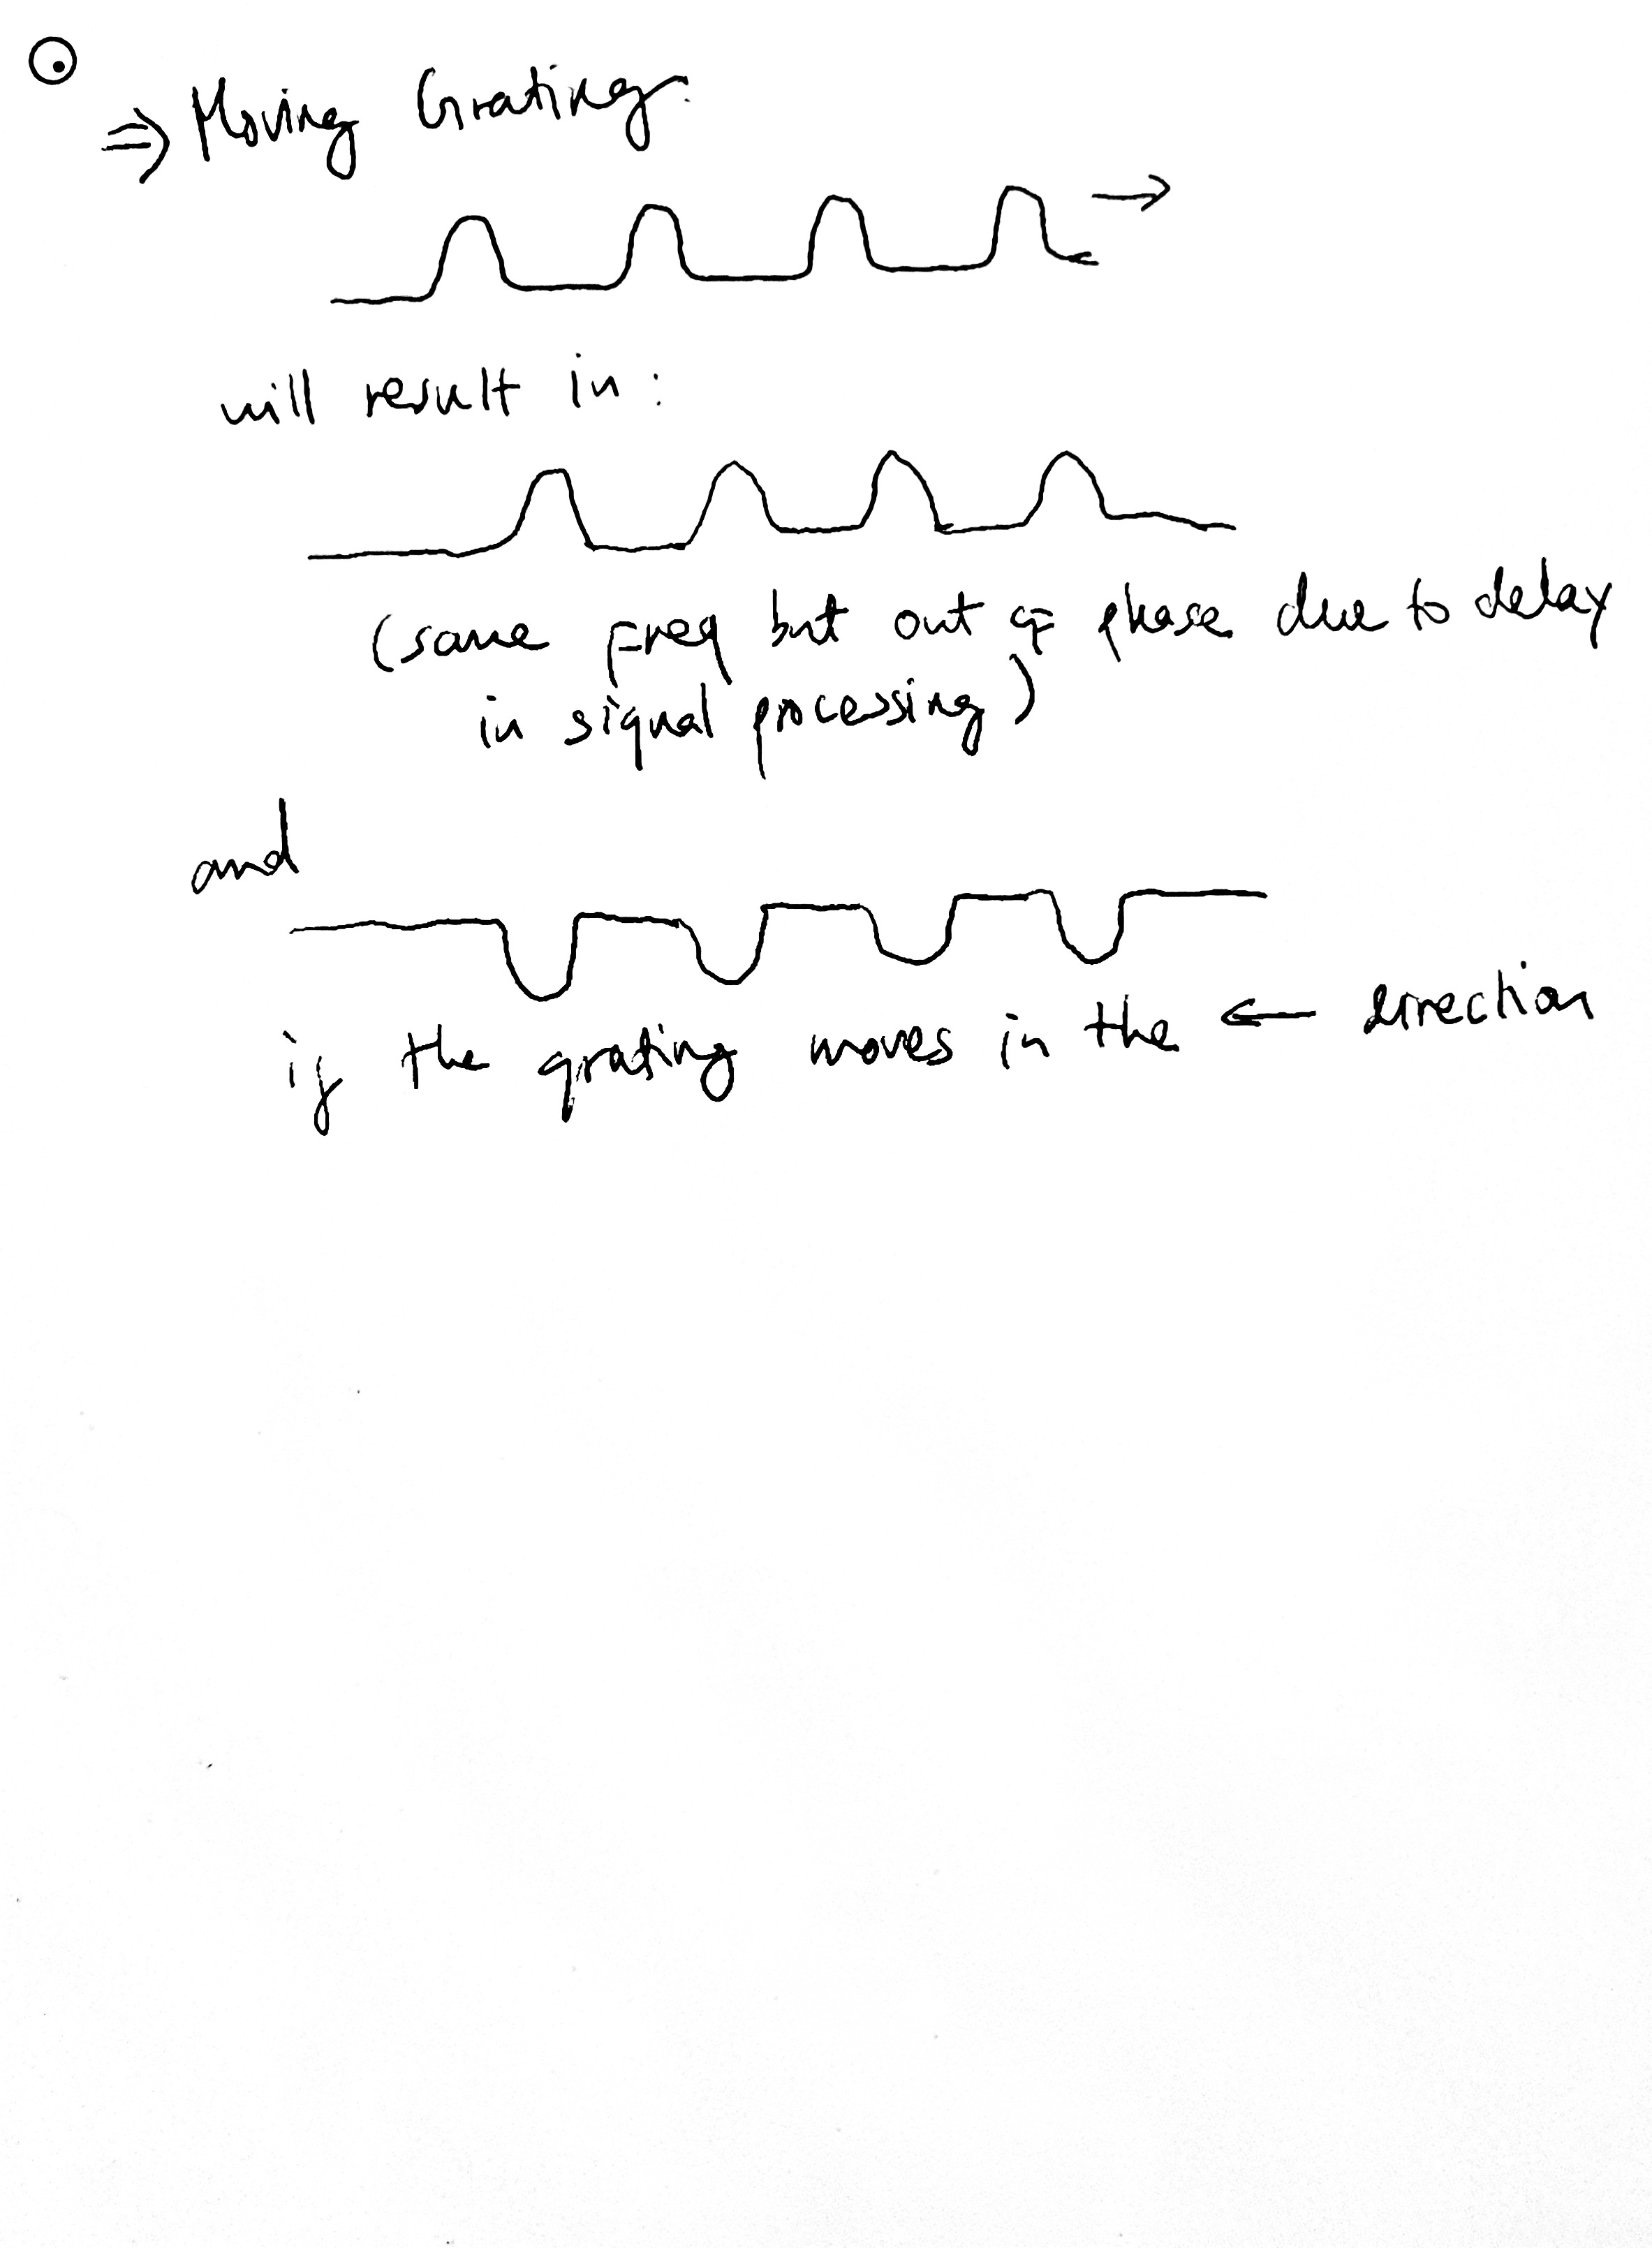
\includegraphics[width=0.7\linewidth]{4c.jpg}
\end{figure}


%\begin{equation}
%Q=\begin{cases}
%1, & \text{Data if rising edge of Clock}.\\
%0, & \text{else keep previous data}
%\end{cases}
%\end{equation}

%\begin{figure}[htb!]
%	\centering
%	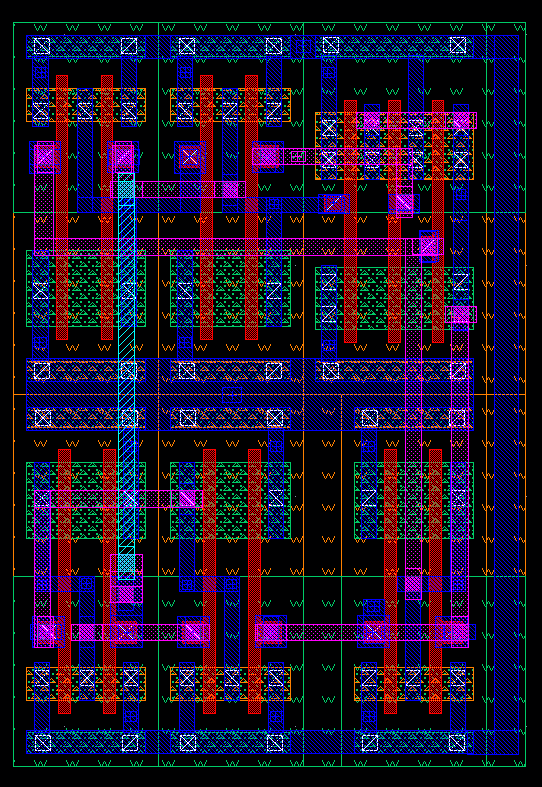
\includegraphics[width=0.6\linewidth]{dff_layout.png}
%	\caption{DFF's Layout in Cadence's Virtuoso Layout Suite}
%	\label{fig8}
%\end{figure}


%\begin{figure}[ht!]
%	\centering
%	\begin{subfigure}[b]{.48\linewidth}
%		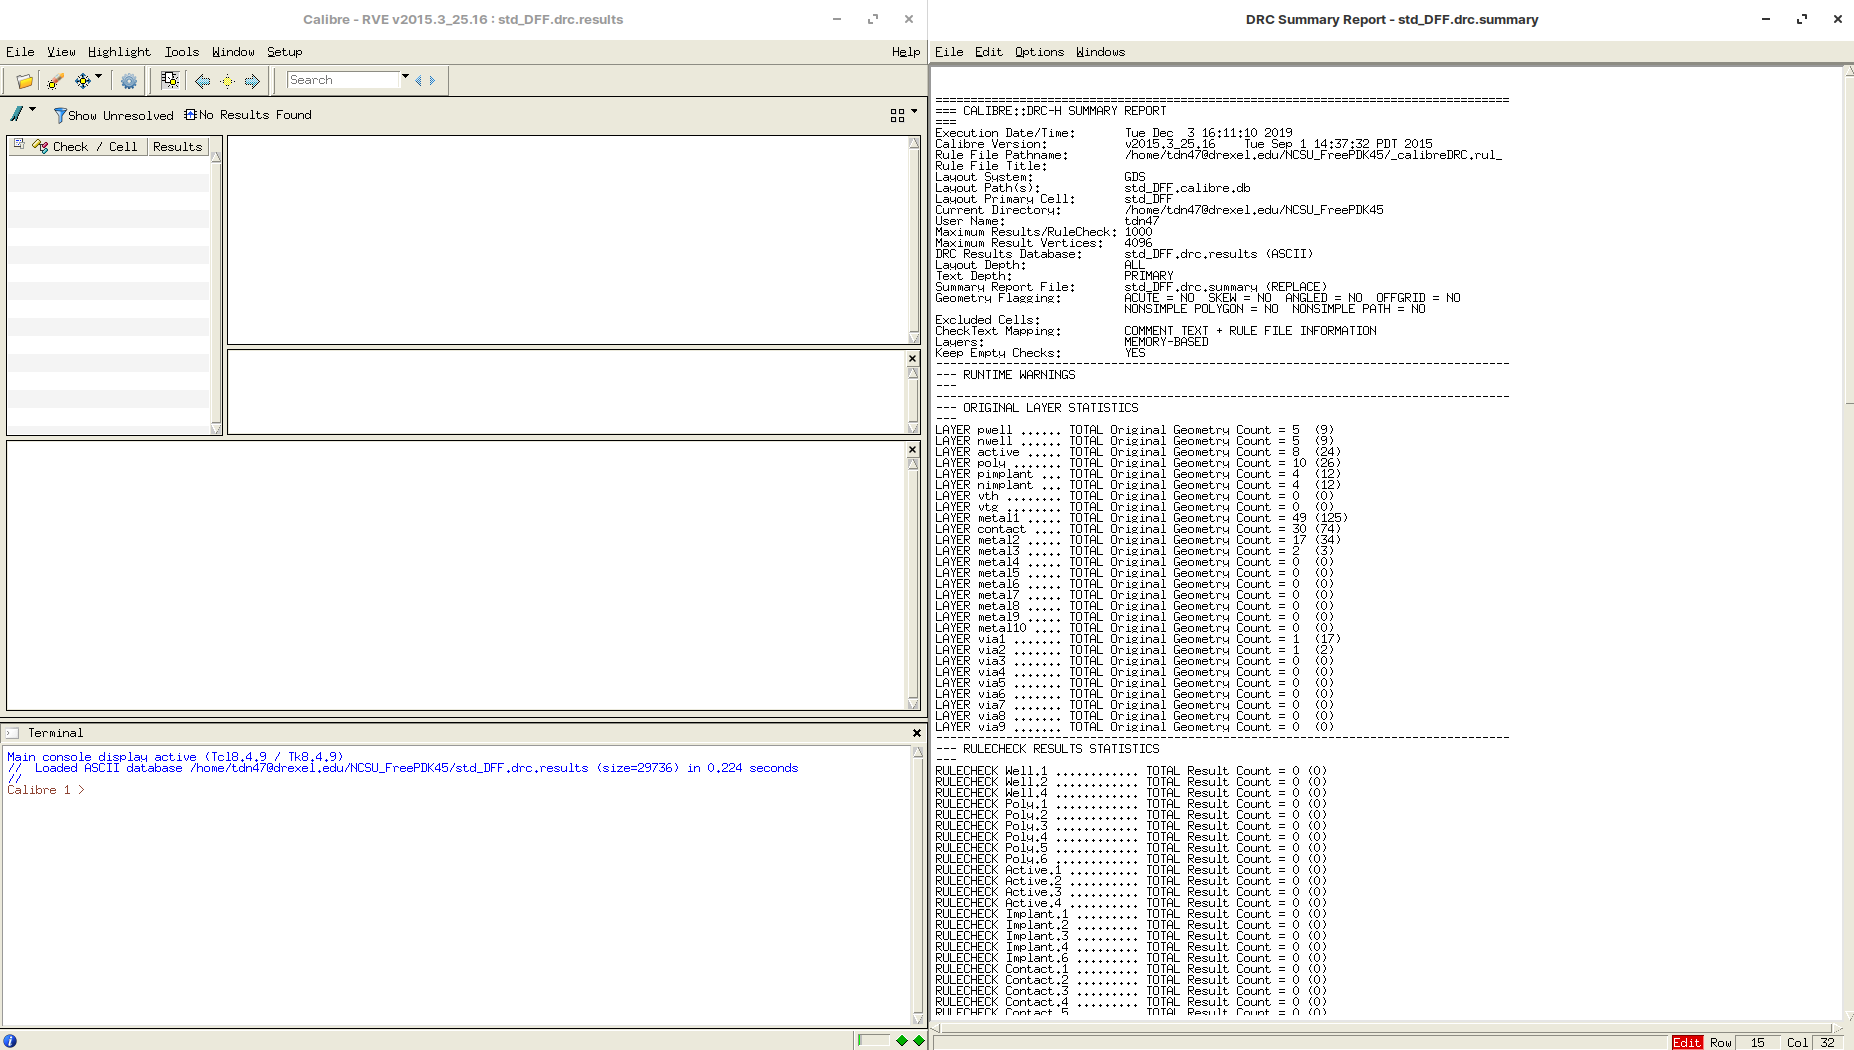
\includegraphics[width=\textwidth]{dff_drc.png}
%		\caption{DFF's rise and fall time}
%		\label{fig9a}
%	\end{subfigure}
%	%	\hskip2em
%	\begin{subfigure}[b]{.48\linewidth}
%		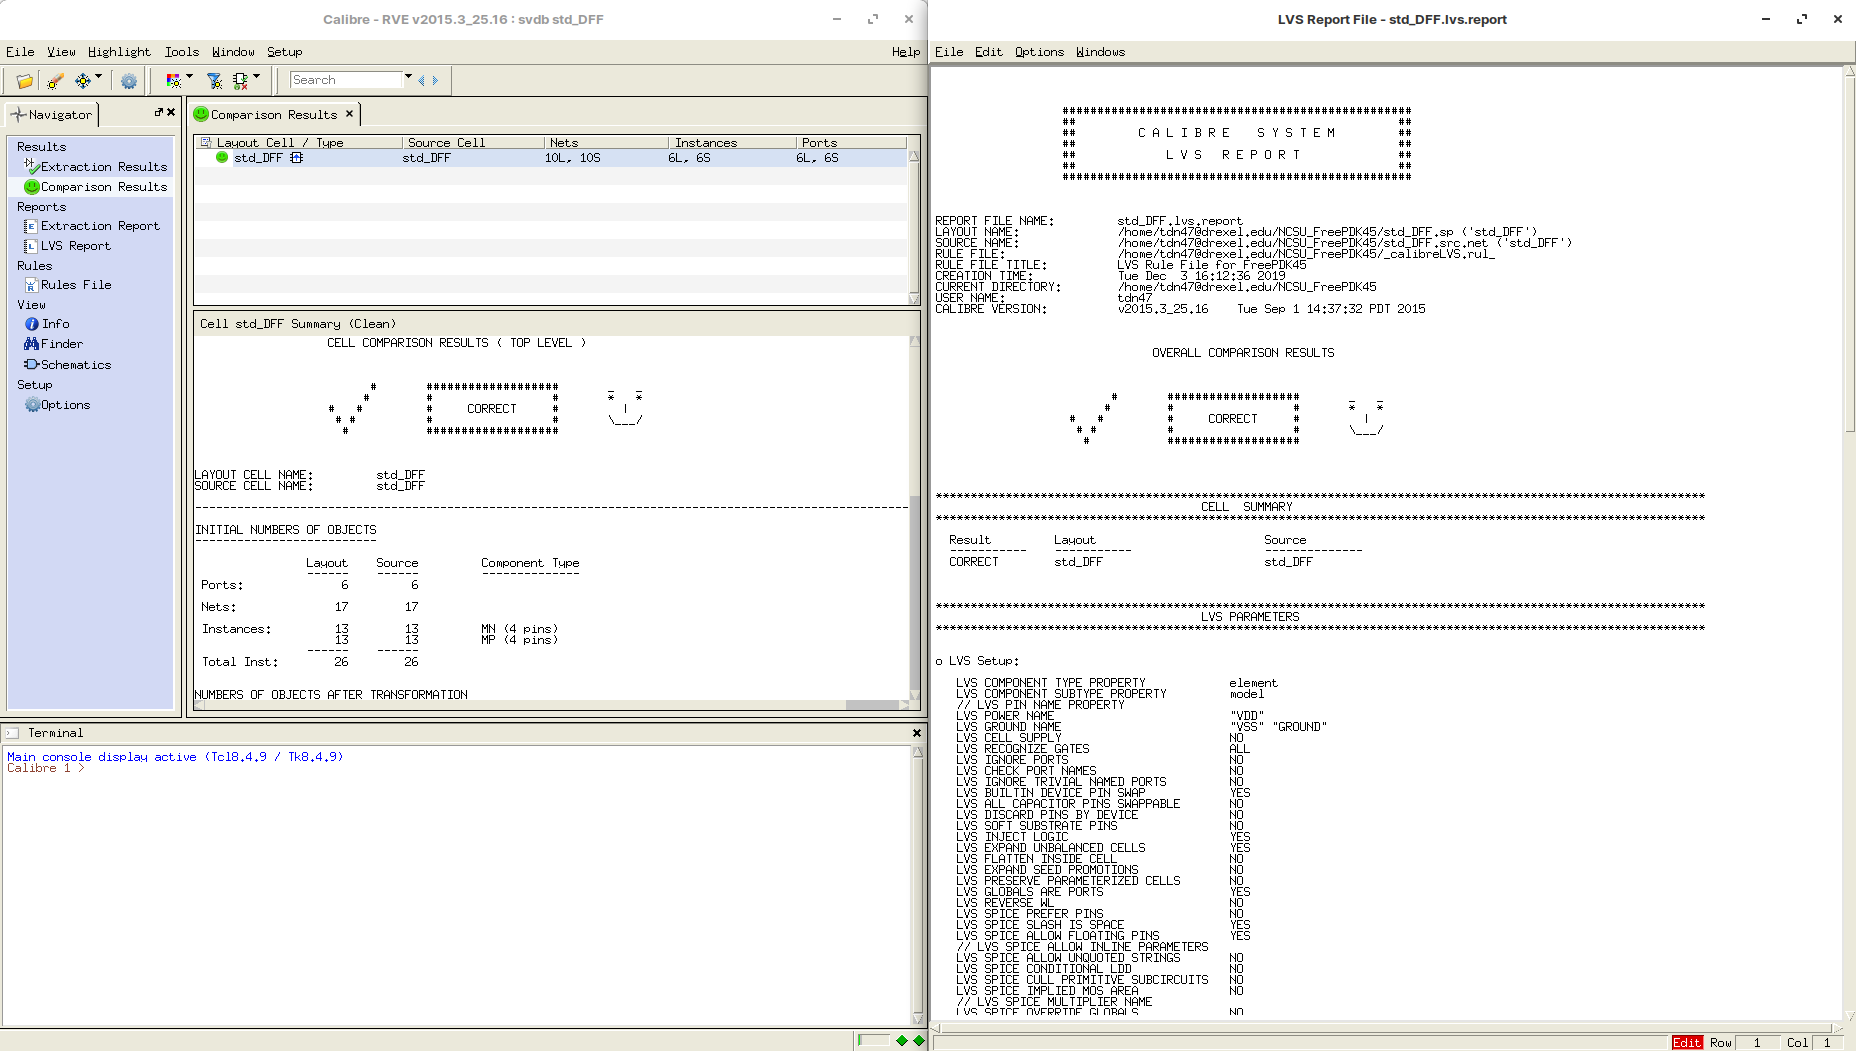
\includegraphics[width=\textwidth]{dff_lvs.png}
%		\caption{DFF's propagation delay}
%		\label{fig9b}
%	\end{subfigure}
%	\caption{Measurements of the DFF's rise/fall time and propagation delay}
%\end{figure}

\end{document}